\documentclass{article}
\usepackage{graphicx}
\graphicspath{{images/}}
\usepackage{float}
\usepackage{hyperref}
\usepackage{authblk}
\title{Introducción a Packet Tracer}
\author{Tomás Gomez

\href{mailto:tomasgomez616@gmail.com}{tomasgomez616@gmail.com}}
\date{August 21, 2024}
\begin{document}

\maketitle


\section{Packet Tracer}

Packet Tracer es una herramienta que permite simular redes reales. 
Proporciona tres menús principales que puede utilizar para lo siguiente:
    \begin{itemize}
        \item Puede agregar dispositivos y conectarlos a través de cables o de forma inalámbrica.
        \item Puede seleccionar, eliminar, inspeccionar, etiquetar y agrupar componentes dentro de la red.
        \item Administrar una red.
    \end{itemize}
Nos permite visualizar la parte logica de la tipologia de forma que podemos observar como se conectan los dispositivos y como fluirán los datos a través de la red.
Y una parte fisica, donde podemos ver como los dispositivos estan distribuidos y conectados.
\\ \\
Nos permite seleccionar componentes de red, tales como routers, servidores, ordenadores, y otros dispositivos para añadir a la topología y explorarlos en detalle, asi como tambien el cableado para conectar estos dispositivos.
\\
También podemos crear paquetes en la red para viajar a través de múltiples dispositivos y poder ver esos paquetes a medida que viajan a través de la red.
\\ \\
Cisco Packet Tracer proporciona dos modos de funcionamiento para visualizar el comportamiento de una red: en tiempo real y modo de simulación.
\\
\\
El Packet Tracer cuenta con pestañas para explorar cada dispositivo, en las cuales encontramos:
   \begin{itemize}
        \item \textbf{Pestaña Física:} La Pestaña Física proporciona una interfaz para interactuar con el dispositivo que incluye encenderlo o apagarlo o instalar diferentes módulos, como una \textit{tarjeta de interfaz de red inalámbrica} (NIC).
        \item \textbf{Pestaña Configuración:} Para los dispositivos intermedios, como enrutadores y conmutadores, hay dos formas de acceder a las configuraciones de los dispositivos. Se puede acceder a las configuraciones a través de la pestaña Config que es una \textit{interfaz gráfica de usuario} (GUI). También se puede acceder a las configuraciones mediante una interfaz de \textit{línea de comandos} (CLI).

La pestaña Configuración no simula la funcionalidad de un dispositivo. Esta pestaña es exclusiva de Packet Tracer. Si no sabe cómo usar la interfaz de línea de comandos, esta pestaña proporciona una forma de usar una GUI exclusiva de Packet Tracer para configurar los ajustes básicos. A medida que se cambian los ajustes en la GUI, los comandos CLI equivalentes aparecen en la ventana Comandos IOS equivalentes. Esto le ayuda a aprender los comandos de la CLI y el \textit{Sistema Operativo de Interconexión de Redes de Cisco} (IOS) mientras utiliza la pestaña Configuración.
        \item \textbf{Pestaña CLI:} La pestaña CLI proporciona acceso a la interfaz de línea de comandos de un dispositivo Cisco. El uso de la pestaña CLI requiere conocimiento de la configuración del dispositivo con IOS. Aquí, puede practicar la configuración de dispositivos Cisco en la línea de comandos. La configuración de CLI es una habilidad necesaria para implementaciones de redes más avanzadas.
        \item \textbf{Pestaña Escritorio:} Para algunos dispositivos finales, como PC y portátiles, Packet Tracer proporciona una interfaz de escritorio que le da acceso a la configuración de IP, la configuración inalámbrica, el símbolo del sistema, un navegador web y otras aplicaciones.
        \item \textbf{Pestaña Servicios:} Un servidor tiene todas las funciones de un host con la adición de una pestaña más, la pestaña Services (Servicios). Esta pestaña permite configurar un servidor con procesos de servidor comunes, como HTTP, DHCP, DNS u otros servicios.
    \end{itemize}

\section{Dispositivos finales}
Los dispositivos finales son aquellos equipos que se conectan a una red y son utilizados por los usuarios para acceder a servicios y recursos. Estos dispositivos son esenciales en la arquitectura de red, ya que representan el punto de interacción entre los usuarios y la infraestructura de red. Entre los mas destacables se encuentran:
\begin{itemize}
    \item \textbf{PC:} Una PC (Computadora Personal) es un dispositivo electrónico diseñado para realizar tareas de procesamiento de datos y facilitar la interacción del usuario. Se utiliza comúnmente en hogares y oficinas para una variedad de aplicaciones. A continuación se detallan sus características principales. Sus componentes principales son: El CPU, la Memoria RAM, el Disco Duro y la Placa Base.
    \item \textbf{Laptops:} Una laptop (o computadora portátil) es un tipo de computadora personal diseñada para ser portátil, lo que significa que se puede llevar fácilmente de un lugar a otro. La pantalla está incorporada en el mismo dispositivo, lo que elimina la necesidad de un monitor externo; Incluyendo además un teclado y un touchpad (o trackpad) para la entrada de datos, todo en un solo dispositivo.
    Cuentan con una batería recargable que permite su uso sin necesidad de estar conectadas a la corriente eléctrica, lo que aumenta su portabilidad.
    \item \textbf{Servidores:} Un servidor es un tipo de computadora o sistema que proporciona servicios, recursos o datos a otras computadoras, conocidas como clientes, a través de una red. Los servidores son fundamentales en la infraestructura de internet y en redes locales. Generalmente cuentan con procesadores más potentes y mayor cantidad de memoria RAM en comparación con las computadoras personales, lo que les permite manejar múltiples solicitudes simultáneamente.\\
    Suelen tener grandes capacidades de almacenamiento para manejar grandes volúmenes de datos y archivos y están diseñados para estar siempre conectados a la red, permitiendo el acceso constante a los recursos que ofrecen.
    \item \textbf{Impresoras:} Una impresora es un dispositivo periférico que permite la producción de copias físicas de documentos, imágenes o gráficos almacenados en una computadora o en un dispositivo móvil. La conexión más común es por medio de USB, permitiendo la conexión directa a una computadora. Aunque también existe la conexión inalambrica (Wi-Fi) que permite la impresión desde dispositivos móviles y computadoras sin necesidad de cables y la conexion por cable Ethernet, que es una conexión a redes locales para compartir impresoras entre varios usuarios.
\end{itemize}

\section{Dispositivos de Red}
Los dispositivos de red son componentes esenciales utilizados para interconectar computadoras y otros dispositivos dentro de una red. Permiten la comunicación, el intercambio de datos y la gestión del tráfico de información. Estos dispositivos pueden variar en función de su función, tipo y tecnología. Los principales dispositivos de red que nos encontramos en la herramienta \textbf{Cisco Packet} Tracer son :
    \begin{itemize}
        \item \textbf{Routers:} Un router es un dispositivo de red que se encarga de dirigir el tráfico de datos entre diferentes redes, como la red local (LAN) y la red de área amplia (WAN) o internet. \\ Los routers son fundamentales para la conectividad de los dispositivos en una red y para el acceso a internet. \\ Permiten la conexión de dispositivos mediante cables por puertos Ethernet o conexiones inalámbricasque proporcionan acceso a internet a dispositivos móviles y computadoras sin necesidad de cables. \\
        Facilitan la conexión de una red local a internet, permitiendo que múltiples dispositivos se conecten a la red global. \\ Posee distintos modelos disponibles: Cisco 1841, 2811, 2911, 819, 829, 1240, PT, 1841, 2620, 2621. Su Firmware esta basado en sistemas operativos IOS (Internetwork Operating System). 
        \\ Y las tarjetas disponibles son : Tarjetas de interfaz WAN (como T1, E1) y 
        tarjetas de interfaz serial.
        
         \item \textbf{Hubs:} Los hubs son dispositivos de red que se utilizan para conectar múltiples dispositivos en una red local (LAN). Cuya función principal es actuar como un punto central de conexión donde los dispositivos pueden comunicarse entre sí. 
         \\ Su uso ha disminuido considerablemente debido a la disponibilidad de dispositivos más avanzados, como switches, que ofrecen un mejor rendimiento y eficiencia en la gestión del tráfico de red. Los modelos que ofrece el Packet Tracer son: Hub-PT, Repeater-PT, CoAxialSplitter-PT.\\ Los Hubs funcionan de manera básica y no tienen configuraciones avanzadas que se asocian con el firmware. El modelo Hub-PT Posee espacio para la posible aplicacion de mas puertos Ethernet en su superficie.
        
        \item \textbf{Switch:} Un switch es un dispositivo de red que conecta múltiples dispositivos dentro de una misma red local (LAN), permitiendo la comunicación entre ellos. A diferencia de los hubs, que simplemente transmiten datos a todos los puertos, los switches son más inteligentes, ya que envían datos solo al dispositivo de destino específico, lo que mejora la eficiencia de la red. \\Los switches pueden tener varios puertos que permiten la conexión de múltiples dispositivos, como computadoras, impresoras y servidores. \\ Los switches pueden filtrar el tráfico de datos, enviando solo la información necesaria al dispositivo correcto, lo que mejora el rendimiento de la red. \\ Entre sus modelos se encuentran : Cisco 2960, 2950, Switch-PT, IE-2000, 3560, 3650. Su Firmware esta basado en Internetwork Operating System Software.\\ Posee la disponibilidad de tarjetas de Módulos de red Ethernet y módulos \textbf{SFP} (Small Form-Factor Pluggable).

        
    \end{itemize}

\section{Cableado}
 El software nos permite probar las diferentes conexiones entre los dispositivos y el cableado correcto y eficiente  para estas conexiones. En un apartado inferior podemos observar los distintos tipos de enlaces entre dispositivos y explorar sus caracteristicas. 
 \\
 Aparecen estas opciones de conexion en el submenu de conexiones: 
 \begin{itemize}
     \item \textbf{Automatically Choose Connection Type}: Nos permite seleccionar automaticamente el cable correcto para enlazar ambos dispositivos.  
     \item \textbf{Console}: Utilizado para conectar un ordenador a un disposivo de red (como un router o switch) para configuración.
     \item \textbf{Serial}: Utilizado para conectar dispositivos de red a través de enlaces seriales (por ejemplo routers).
     \item \textbf{Coaxial}: Se utiliza para algunas redes antiguas y conexiones de televisión.
     \item \textbf{Fiber}: Para conexiones de alta velocidad y largas distancias.
     \item \textbf{Crossover}: Utilizado para conectar dispositivos similares, como un switch a otro switch o un PC a otro PC.
     \item \textbf{Straight-Throught}: Para conectar dispositivos diferentes, como un switch a un PC.
 \end{itemize}

 
 \section{Actividad práctica interconectando dos PCs}
Como podemos observar en la figura la conexión entre las dos PC's se da mediante el uso de un cable \textit{Cross-over} ya que son dispositivos similares entre si.
    \begin{figure}[H]
        \centering
        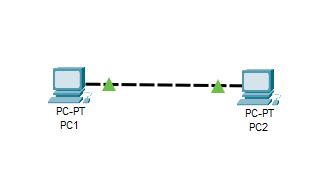
\includegraphics{PacketTracer_bNPPSspTGp.png}
        \caption{Dos PC's conectadas entre si.}
        \label{fig:figura 1}
    \end{figure}

Lo que podemos analizar es que al solo poder conectar dos computadoras simultaneamente mediante un cable, nos da la limitación de no poder extender este enlace a una máquina más. 
\\Podemos llegar a la conclusión que debido a este inconveniente lograron surgir varias implementaciones como la creación de los Hubs, o switchs para poder hacer posible que un tercer dispositivo pueda establecer su conexión con estas dos computadoras.
     \begin{figure}[H]
        \centering
        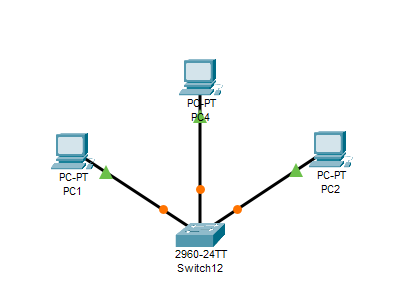
\includegraphics{PacketTracer_25tnBqSEIw.png}
        \caption{Tres PC's conectadas a un mismo switch. }
        \label{fig:figura 2}
    \end{figure}

\section{Referencias}
\begin{itemize}
    \item \href{https://skillsforall.com/course/getting-started-cisco-packet-tracer?utm_source=netacad.com&utm_medium=referral&utm_campaign=packet-tracer&courseLang=es-XL&userlogin=0}{Introducción a Cisco Packet Tracer}

    \item \href{https://www.opera.com/es-419/features/aria} {Inteligencia artificial Aria}

    \item Software Cisco Packet Tracer. \href{https://www.netacad.com/es/courses/packet-tracer}{Link de descarga}
    
    \item Fuente del documento: \href{https://github.com/tomyygun/Packet-Tracer-Actividad-1}{https://github.com/tomyygun/Packet-Tracer-Actividad-1}
\end{itemize}


\end{document}


